\documentclass[letterpaper,12pt]{article}   %%% Can be report

%% set paper margins
\oddsidemargin=0.1in
\evensidemargin=0.1in
\textwidth=6.0in
\topmargin=-0.7in
\textheight=9.0in
\parindent=0.2in

\usepackage{amsmath,amssymb,bm}
\usepackage{graphicx}
\usepackage{rotating}
\usepackage{subfigure}
\graphicspath{%
  {figs/ipe/}
  {figs/dia/}
  {figs/matlab/}
  {figs/imag/}
} 
\usepackage[width=11cm,font=footnotesize,labelfont=bf, %
format=default,justification=centerlast]{caption} % Figure caption text customization 

\usepackage{pgfgantt}

\usepackage{booktabs,array} % Packages for tables

\usepackage{hyperref}
\usepackage{soul}
\usepackage{setspace}
\usepackage{multirow}

\usepackage[ruled, vlined, linesnumbered]{algorithm2e} % For algorithms

\usepackage{tikz}
\usetikzlibrary{positioning,fit}

\usepackage{siunitx}
\sisetup{unitsep=\cdot}

\title{ECE498:~Senior Capstone Project I\\\textbf{\underline{Project Proposal}}\\
\vspace{0.5in}
Project Title: Robotic Cart
\vspace{1.0in}
\author{Kallistah Allen, Darrah Beebe and Jason Braker\\ Advisors: Dr.~Suruz Miah and Dr.~Prasad Shastry}
}
%\date{February 6, 2003}  No need to write, Date will be automatically on the title page
\date{}  % Do not show date on the title page

%%%%%%%%%%%%%%%%% Set document line spacing %%%%%%%%%%%%%%%%%%%%%
\singlespacing
%\onehalfspacing
%\doublespacing
% all packages are in the following tex file.
%\input{paper-preamble.tex}
\begin{document}

%%% Make title page 
\begin{titlepage}
 \maketitle

\vspace*{4.0cm}
\begin{center}
\normalsize
Electrical and Computer Engineering Department\\
Caterpillar College of Engineering and Technology\\
\href{http://www.bradley.edu/}{Bradley University}\\

\vspace*{6.0cm}
\copyright~K.~Allen,~D.~Beebe~and~J.~Braker, Peoria, IL, USA, 2020\\

\end{center}
\thispagestyle{empty}

\end{titlepage} 
%%%%%%%%%%%%
%\thispagestyle{empty}
%\maketitle
\newpage
\renewcommand{\contentsname}{Table of Contents}
\tableofcontents
\newpage

\section{Introduction} %introduction (basically what was in the project description before)


Robotic carts are a prevailing invention designed to aid the customer in a number of important indoor and outdoor tasks. There are systems currently on the market that perform these tasks in a variety of ways. For example, in a grocery store, a customer may require the need of more than one cart but cannot push or pull two carts simultaneously. One major drawback however is that people with disabilities cannot push one cart let alone have a second cart to carry more items. In this project, we are proposing a robotic cart that would primarily use analog signals with the use of cost-effective wireless communication to identify the customer and be able to track and follow the customer through the store. This implementation of a fully functional robotic cart will outreach the scope of the project but is the overall goal for this project in the coming years while encouraging further research into this field. Applications of this system include mail delivery carts, file transferring carts in offices, hospital carts to aid nurses and doctors by carrying medicine or surgery supplies, and use in construction sites to carry tools and other supplies across the job site.

\section{Literature Review} %review of literature and prior work

Abounding research in the field of robotic carts shows various ways in which to implement a system that will help consumers with carrying groceries through stores (see~\cite{Rawashdeh2017-Person},~\cite{islam_lam_fukuda_kobayashi_kuno_2019},~\cite{Sales2016-CompaRob}). Currently, the work being done focuses on a few different methods of having the robotic cart interface with the customer and follow them through the store. A mobile platform interface that implements ultrasound and radio transmissions technology is one such method that has been utilized to follow a customer through a store~\cite{Sales2016-CompaRob}. Another method that has been implemented is the use of a GRU (Gated Recurrent Unit) network to detect shopping habits of customers while also using a LiDAR sensor and camera to detect and map the customer using a two-dimensional skeleton and follow them through the store~\cite{islam_lam_fukuda_kobayashi_kuno_2019}. In the last method, the authors utilized an Arduino MEGA 2560, six ultrasonic sensors, two DC motors with PWM (Pulse Width Modulation), an Android Studio IDE device, and Bluetooth in order to detect the customer and follow them through the store~\cite{Rawashdeh2017-Person}. In our project we are implementing XBee S2C RF radios, which are inexpensive and easily configurable, as a remote that the robot will be able to track instead of using line of sight methods~\cite{Miah2018-Intelligent}. In addition with the XBee S2C RF radios we will equip the robot with a parabolic reflector, which improves Wi-Fi reception at various distances and angles, based on research done previously in this type of robot localization and mapping~\cite{Miah2018-Intelligent}~\cite{Li2013ANA}. This approach also requires understanding of multipath interference which is common in Wi-Fi based wireless positioning sensing systems. Some methods, seen in~\cite{xie_jiang_zhao_zhang_2019}, explains that using course estimation calculations such as received signal strength indicator (RSSI) and time difference of arrival (TDoA) is key to compensate for the multipath interference in received signals.~\cite{ladd_bekris_rudys_kavraki_wallach_2005} shows a different approach to the multipath issue by using an IEEE 802.11b wireless Ethernet device to measure RF signals. This device system was used because it is communicable between a mobile device and a localization based service with low complexity for the user. Also, in~\cite{lindhe_johansson_bicchi_2007} the research states several other ways to counteract the multipath fading with methods such as antenna diversity, frequency spreading, or adaptive antenna arrays. The method used in this paper was to sample the radio signal strength (RSS) at discrete points without too much deviation from the robot's desired position in an indoor environment. Lastly, in~\cite{Lindhe2009} the method that is utilized exploits multipath fading by measuring the signal-to-noise ratio (SNR) and adjusting the robot's motion to spend more time where the channel strength is greater.

\vspace*{12pt}
In this project we aim to use the XBee S2C RF radios and a parabolic reflector combined into a rotating system similar to the one presented in~\cite{Miah2018-Intelligent} in order to have the robot track the customer through a store. The major challenges of this implementation will be the communication between the robot and the remote as well as maintaining a buffer distance between the robotic cart and the customer without using line of sight sensing.


% \section{Standards and Patents}
% The standards that are applicable to our project include the IEEE 802.15.4 protocol and the ZigBee protocol. The IEEE 802.15.4 protocol\footnote{IEEE Standard for Low-Rate Wireless Networks, 2015} outlines the physical layer (PHY) and the medium access control layer (MAC) specifications for low-data-rate wireless communication in personal area networks (LR-WPAN). The PHY layer contains the radio frequency transceiver and its low-level controller. The MAC layer provides access to the physical channel for transfer and defines an IEEE address for the device. Its goal is to maintain a simple and flexible protocol while also being easy to install, having reliable data transfer, being low cost, and having reasonable battery life. The ceiling mounted beacons will use XBee modules to communicate wirelessly with the mobile robot and uses the 802.15.4 protocol by default. The 802.15.4 protocol allows for a star network topology which is made up of one established personal area network (PAN) coordinator and other functional devices. In our system, the XBee mounted on the mobile robot will act as a coordinator and the ceiling mounted XBee’s will be the other functional devices. During our testing, we have established basic peer-to-peer communication with this protocol.\\

% The other standard known as ZigBee\footnote{Zigbee Pro Stack User Guide, 2014}\footnote{XBee/XBee-Pro S2C ZigBee User Guide, 2016} is an open global standard for low-power, low-cost, low-data-rate, wireless networking based on the IEEE 802.15.4 standard. It maintains the specifications of the PHY layer and the MAC layer while defining the higher network layer and setting the framework for the application layer. The network layer takes care of network structure, routing, and security. The application layer has an application support sub-layer (APS) which defines various addressing objects and has other features for device specific applications. The ZigBee protocol allows for star, peer-to-peer, and mesh network topologies. We will still use the star network topology which is made up of a coordinator who creates a network with a channel and a unique PAN ID and end devices who will join this network with extra power saving features. The XBee mounted on the mobile robot will act as the coordinator and the ceiling mounted beacons will act as the end devices. The fully functional system will be implemented with a ZigBee network. It offers well defined packetized communication, power saving features which is important for the battery powered ceiling mounted beacons, and future applications which may require a higher level mesh network.\\

% There are several patents that outline designs that are comparable to our project. The first patent~\cite{biehl} describes systems and methods for localization of a mobile device using beacons. This design uses a computer, a location signal receiver and beacons to determine the location of the mobile device. The beacons transmit the location signal and  the computer determines the location from the received location signal strength and a unique key based on the particular transmitting beacon. This patent is relevant to our work as it uses received signal strength from beacons and individual beacon IDs for localization of a mobile device in an indoor environment, but the patent is more general to what the mobile device is and uses a different localization algorithm. The second patent~\cite{lin} outlines positioning of an indoor mobile robot, and mapping of its environment and the beacons it detects. The mobile robot performs several positioning modes depending on the number on beacons it detects in its line of sight. This patent is more applicable to our project than the last patent. It utilizes a simultaneous localization and mapping technique for a mobile robot and beacons. However, the patent's positioning method is different than ours. The third patent~\cite{edlund} describes a localization method for a mobile robot with a system of beacons. It uses the signal strength and angle of arrival of the signal to localize and determine a coarse correction. This design is very similar to our approach by uses signal strength and angle, and similar localization algorithm, but we will be rotating a antennae reflector instead of the entire robot. A similar patent~\cite{younis} to the previous explains an indoor localization method for a mobile device using directional reflectors. The mobile device transmits a signal and the signal is delayed and returned by reflectors in the environment. The location of the mobile device is then determined from the range by the amount of delay and the angle of arrival at the reflector. This patent is relatively similar to our project as it describes an indoor localization technique using range and angle for a mobile device.

\section{Functional Requirements}
\subsection{System Architecture}
\hspace{\parindent} The system for this project consists of two subsystems which are the Mobile Cart and the Remote Target as seen in Figure \ref{fig:sys_block_diag}. The Mobile Cart system is a mobile wheeled robot that sends and receives radio signals to follow a target. The Remote Target acts as the target for the Mobile Cart in the system by sending radio signals back and forth with the cart.

\begin{figure}[!h]
    \centering
    
\includegraphics[scale=0.9]{figs/system_block_diagram_2}
    \caption{System level block diagram detailing inputs and outputs to the system}
	\label{fig:sys_block_diag}
\end{figure}

\vspace*{12pt}
\subsection{Block Diagrams}
\hspace{\parindent} Both subsystems of this project, being the Mobile Cart and Remote Target, act as their own enclosed systems, only relaying radio messages between them. For the Remote Target subsystem, Figure \ref{fig:remote_block_diag} contains the block diagram for it. Of the two subsystems the Remote Target is the simplest since it only is requires an XBee module attached to a 9 volt battery.

\hspace{\parindent} The Mobile Cart section of the system is shown as a block diagram in Figure \ref{fig:remote_block_diag}. The Mobile Cart for inputs consists of Power coming from a Li-Po battery toggled by a On/Off switch, buttons for changing carts operating mode, and messages received from the remote target. The Mobile Cart works off of a central controller, which is the BeagleBone Blue, DC Motors for the driving of the cart as well as a stepper motor used for the radio sensor array, and a sensor array consisting of one omnidirectional transmitter and 4 directional receivers. The transmitters and receivers are all XBee modules connected to the central BeagleBone Blue which are used in tandem along with the stepper motor to check signal strength with the Remote Target.

\begin{figure}[!h]
    \centering
    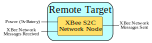
\includegraphics[scale=0.9]{figs/remote_target_block_diagram}
    \caption{Remote Target block diagram}
	\label{fig:remote_block_diag}
\end{figure}
\begin{figure}[!h]
    \centering
    \includegraphics[scale=0.82]{figs/mobile_cart_block_diagram}
    \caption{Mobile Robot block diagram}
	\label{fig:mobile_block_diag}
\end{figure}

\subsection{Navigation Algorithm}
We will use a modified Point Navigation algorithm to navigate the robot to follow the remote. The robot will estimate the coordinates of the remote with respect to the robot's local reference frame. The robot will then apply actuation to move to the point that is a set following distance from the remote. A high-level flowchart of the algorithm is shown in \autoref{fig:navAlgoFlowchart}. Also, a pseudo-code version of the algorithm is shown in \autoref{alg:navAlgo}.

\begin{figure}
  \centering
  % Graphic for TeX using PGF
% Title: S:\Senior Project\seniorProject2-2020-21-Docs\figs\dia\algorithmFlowchart.dia
% Creator: Dia v0.97.2
% CreationDate: Thu Nov 19 10:16:16 2020
% For: Jason Braker
% \usepackage{tikz}
% The following commands are not supported in PSTricks at present
% We define them conditionally, so when they are implemented,
% this pgf file will use them.
\ifx\du\undefined
  \newlength{\du}
\fi
\setlength{\du}{15\unitlength}
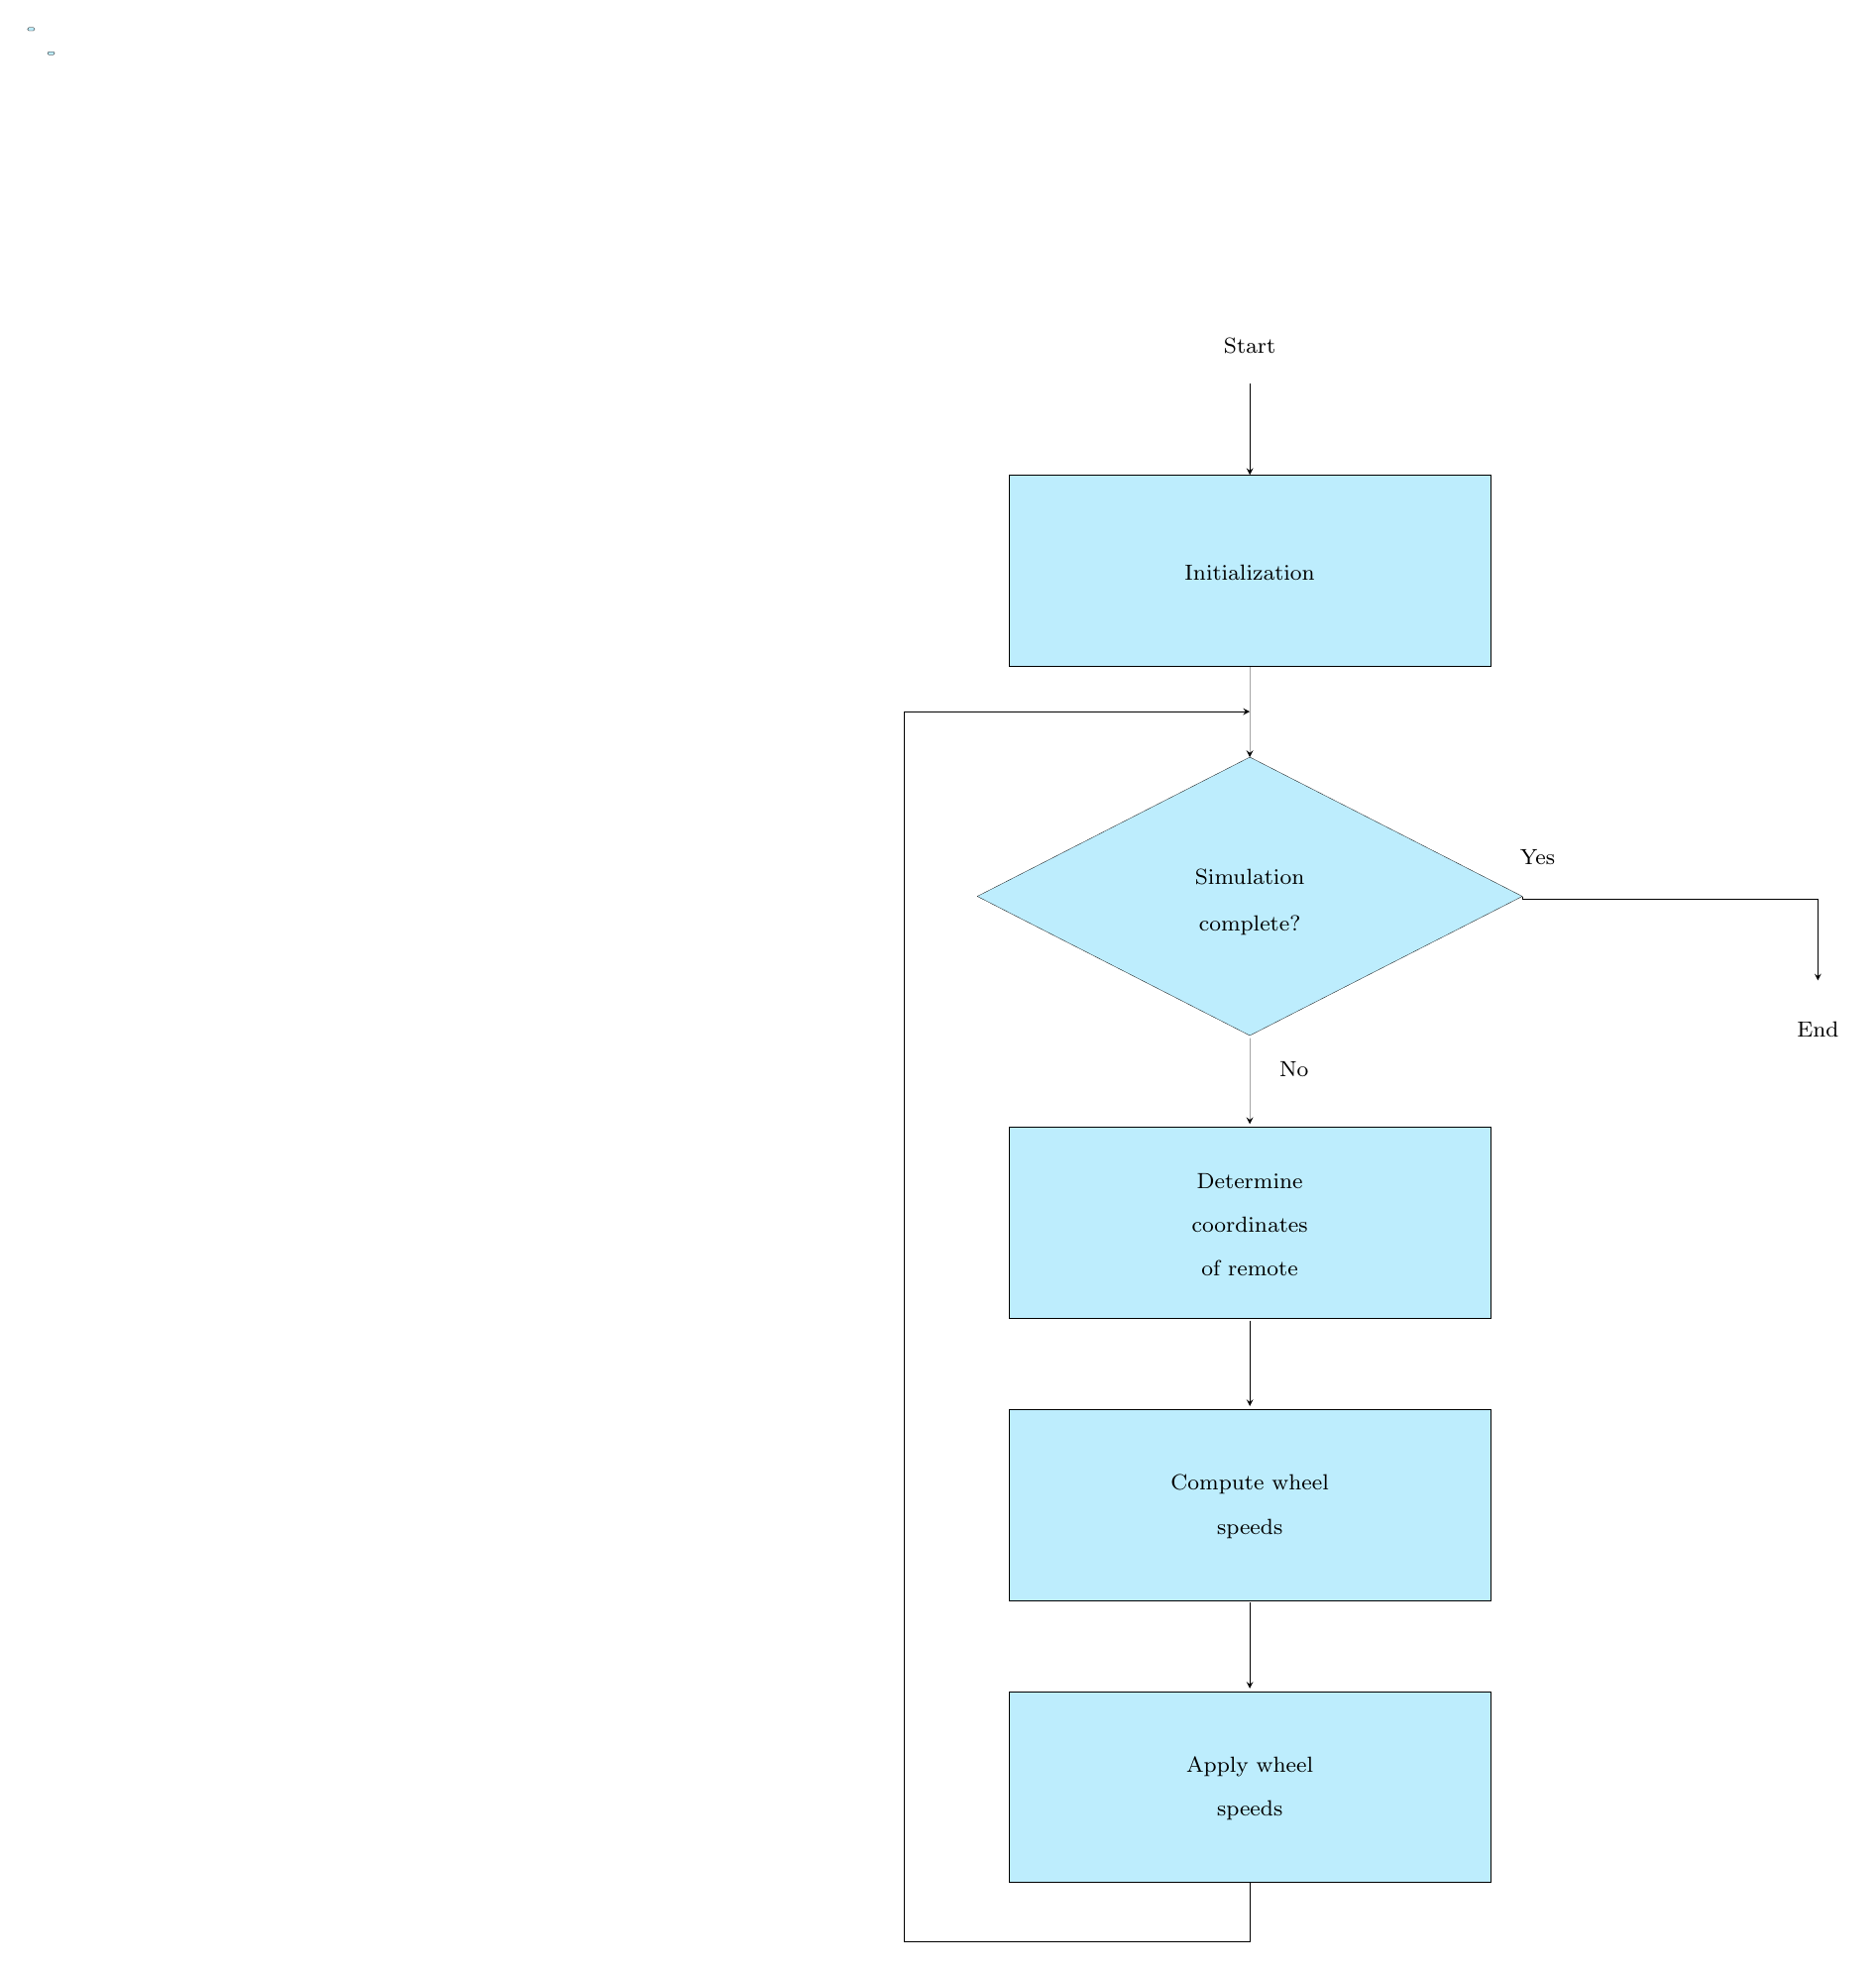
\begin{tikzpicture}[scale=0.7, font=\footnotesize]
\pgftransformxscale{1.000000}
\pgftransformyscale{-1.000000}
\definecolor{dialinecolor}{rgb}{0.000000, 0.000000, 0.000000}
\pgfsetstrokecolor{dialinecolor}
\definecolor{dialinecolor}{rgb}{1.000000, 1.000000, 1.000000}
\pgfsetfillcolor{dialinecolor}
\pgfsetlinewidth{0.100000\du}
\pgfsetdash{}{0pt}
\pgfsetdash{}{0pt}
\pgfsetbuttcap
\pgfsetmiterjoin
\pgfsetlinewidth{0.100000\du}
\pgfsetbuttcap
\pgfsetmiterjoin
\pgfsetdash{}{0pt}
\definecolor{dialinecolor}{rgb}{0.741176, 0.929412, 0.992157}
\pgfsetfillcolor{dialinecolor}
\pgfpathmoveto{\pgfpoint{21.890567\du}{5.100000\du}}
\pgfpathlineto{\pgfpoint{24.357233\du}{5.100000\du}}
\pgfpathcurveto{\pgfpoint{24.697809\du}{5.100000\du}}{\pgfpoint{24.973900\du}{5.458172\du}}{\pgfpoint{24.973900\du}{5.900000\du}}
\pgfpathcurveto{\pgfpoint{24.973900\du}{6.341828\du}}{\pgfpoint{24.697809\du}{6.700000\du}}{\pgfpoint{24.357233\du}{6.700000\du}}
\pgfpathlineto{\pgfpoint{21.890567\du}{6.700000\du}}
\pgfpathcurveto{\pgfpoint{21.549991\du}{6.700000\du}}{\pgfpoint{21.273900\du}{6.341828\du}}{\pgfpoint{21.273900\du}{5.900000\du}}
\pgfpathcurveto{\pgfpoint{21.273900\du}{5.458172\du}}{\pgfpoint{21.549991\du}{5.100000\du}}{\pgfpoint{21.890567\du}{5.100000\du}}
\pgfusepath{fill}
\definecolor{dialinecolor}{rgb}{0.000000, 0.000000, 0.000000}
\pgfsetstrokecolor{dialinecolor}
\pgfpathmoveto{\pgfpoint{21.890567\du}{5.100000\du}}
\pgfpathlineto{\pgfpoint{24.357233\du}{5.100000\du}}
\pgfpathcurveto{\pgfpoint{24.697809\du}{5.100000\du}}{\pgfpoint{24.973900\du}{5.458172\du}}{\pgfpoint{24.973900\du}{5.900000\du}}
\pgfpathcurveto{\pgfpoint{24.973900\du}{6.341828\du}}{\pgfpoint{24.697809\du}{6.700000\du}}{\pgfpoint{24.357233\du}{6.700000\du}}
\pgfpathlineto{\pgfpoint{21.890567\du}{6.700000\du}}
\pgfpathcurveto{\pgfpoint{21.549991\du}{6.700000\du}}{\pgfpoint{21.273900\du}{6.341828\du}}{\pgfpoint{21.273900\du}{5.900000\du}}
\pgfpathcurveto{\pgfpoint{21.273900\du}{5.458172\du}}{\pgfpoint{21.549991\du}{5.100000\du}}{\pgfpoint{21.890567\du}{5.100000\du}}
\pgfusepath{stroke}
% setfont left to latex
\definecolor{dialinecolor}{rgb}{0.000000, 0.000000, 0.000000}
\pgfsetstrokecolor{dialinecolor}
\node at (23.123900\du,6.00000\du){Start};
\definecolor{dialinecolor}{rgb}{0.741176, 0.929412, 0.992157}
\pgfsetfillcolor{dialinecolor}
\fill (23.123842\du,13.536900\du)--(28.113283\du,16.085084\du)--(23.123842\du,18.633268\du)--(18.134400\du,16.085084\du)--cycle;
\pgfsetlinewidth{0.100000\du}
\pgfsetdash{}{0pt}
\pgfsetdash{}{0pt}
\pgfsetmiterjoin
\definecolor{dialinecolor}{rgb}{0.000000, 0.000000, 0.000000}
\pgfsetstrokecolor{dialinecolor}
\draw (23.123842\du,13.536900\du)--(28.113283\du,16.085084\du)--(23.123842\du,18.633268\du)--(18.134400\du,16.085084\du)--cycle;
% setfont left to latex
\definecolor{dialinecolor}{rgb}{0.000000, 0.000000, 0.000000}
\pgfsetstrokecolor{dialinecolor}
\node at (23.123842\du,15.725084\du){Simulation};
% setfont left to latex
\definecolor{dialinecolor}{rgb}{0.000000, 0.000000, 0.000000}
\pgfsetstrokecolor{dialinecolor}
\node at (23.123842\du,16.625084\du){complete?};
\definecolor{dialinecolor}{rgb}{0.741176, 0.929412, 0.992157}
\pgfsetfillcolor{dialinecolor}
\fill (18.709600\du,20.301700\du)--(18.709600\du,23.801700\du)--(27.538230\du,23.801700\du)--(27.538230\du,20.301700\du)--cycle;
\pgfsetlinewidth{0.100000\du}
\pgfsetdash{}{0pt}
\pgfsetdash{}{0pt}
\pgfsetmiterjoin
\definecolor{dialinecolor}{rgb}{0.000000, 0.000000, 0.000000}
\pgfsetstrokecolor{dialinecolor}
\draw (18.709600\du,20.301700\du)--(18.709600\du,23.801700\du)--(27.538230\du,23.801700\du)--(27.538230\du,20.301700\du)--cycle;
% setfont left to latex
\definecolor{dialinecolor}{rgb}{0.000000, 0.000000, 0.000000}
\pgfsetstrokecolor{dialinecolor}
\node at (23.123915\du,21.291700\du){Determine};
% setfont left to latex
\definecolor{dialinecolor}{rgb}{0.000000, 0.000000, 0.000000}
\pgfsetstrokecolor{dialinecolor}
\node at (23.123915\du,22.091700\du){coordinates};
% setfont left to latex
\definecolor{dialinecolor}{rgb}{0.000000, 0.000000, 0.000000}
\pgfsetstrokecolor{dialinecolor}
\node at (23.123915\du,22.891700\du){of remote};
\pgfsetlinewidth{0.100000\du}
\pgfsetdash{}{0pt}
\pgfsetdash{}{0pt}
\pgfsetbuttcap
\pgfsetmiterjoin
\pgfsetlinewidth{0.100000\du}
\pgfsetbuttcap
\pgfsetmiterjoin
\pgfsetdash{}{0pt}
\definecolor{dialinecolor}{rgb}{0.741176, 0.929412, 0.992157}
\pgfsetfillcolor{dialinecolor}
\pgfpathmoveto{\pgfpoint{32.290567\du}{17.675000\du}}
\pgfpathlineto{\pgfpoint{34.757233\du}{17.675000\du}}
\pgfpathcurveto{\pgfpoint{35.097809\du}{17.675000\du}}{\pgfpoint{35.373900\du}{18.033172\du}}{\pgfpoint{35.373900\du}{18.475000\du}}
\pgfpathcurveto{\pgfpoint{35.373900\du}{18.916828\du}}{\pgfpoint{35.097809\du}{19.275000\du}}{\pgfpoint{34.757233\du}{19.275000\du}}
\pgfpathlineto{\pgfpoint{32.290567\du}{19.275000\du}}
\pgfpathcurveto{\pgfpoint{31.949991\du}{19.275000\du}}{\pgfpoint{31.673900\du}{18.916828\du}}{\pgfpoint{31.673900\du}{18.475000\du}}
\pgfpathcurveto{\pgfpoint{31.673900\du}{18.033172\du}}{\pgfpoint{31.949991\du}{17.675000\du}}{\pgfpoint{32.290567\du}{17.675000\du}}
\pgfusepath{fill}
\definecolor{dialinecolor}{rgb}{0.000000, 0.000000, 0.000000}
\pgfsetstrokecolor{dialinecolor}
\pgfpathmoveto{\pgfpoint{32.290567\du}{17.675000\du}}
\pgfpathlineto{\pgfpoint{34.757233\du}{17.675000\du}}
\pgfpathcurveto{\pgfpoint{35.097809\du}{17.675000\du}}{\pgfpoint{35.373900\du}{18.033172\du}}{\pgfpoint{35.373900\du}{18.475000\du}}
\pgfpathcurveto{\pgfpoint{35.373900\du}{18.916828\du}}{\pgfpoint{35.097809\du}{19.275000\du}}{\pgfpoint{34.757233\du}{19.275000\du}}
\pgfpathlineto{\pgfpoint{32.290567\du}{19.275000\du}}
\pgfpathcurveto{\pgfpoint{31.949991\du}{19.275000\du}}{\pgfpoint{31.673900\du}{18.916828\du}}{\pgfpoint{31.673900\du}{18.475000\du}}
\pgfpathcurveto{\pgfpoint{31.673900\du}{18.033172\du}}{\pgfpoint{31.949991\du}{17.675000\du}}{\pgfpoint{32.290567\du}{17.675000\du}}
\pgfusepath{stroke}
% setfont left to latex
\definecolor{dialinecolor}{rgb}{0.000000, 0.000000, 0.000000}
\pgfsetstrokecolor{dialinecolor}
\node at (33.523900\du,18.515000\du){End};
\pgfsetlinewidth{0.100000\du}
\pgfsetdash{}{0pt}
\pgfsetdash{}{0pt}
\pgfsetbuttcap
{
\definecolor{dialinecolor}{rgb}{0.000000, 0.000000, 0.000000}
\pgfsetfillcolor{dialinecolor}
% was here!!!
\pgfsetarrowsend{stealth}
\definecolor{dialinecolor}{rgb}{0.000000, 0.000000, 0.000000}
\pgfsetstrokecolor{dialinecolor}
\draw (23.123900\du,6.700000\du)--(23.123900\du,8.368440\du);
}
\pgfsetlinewidth{0.100000\du}
\pgfsetdash{}{0pt}
\pgfsetdash{}{0pt}
\pgfsetbuttcap
{
\definecolor{dialinecolor}{rgb}{0.000000, 0.000000, 0.000000}
\pgfsetfillcolor{dialinecolor}
% was here!!!
\pgfsetarrowsend{stealth}
\definecolor{dialinecolor}{rgb}{0.000000, 0.000000, 0.000000}
\pgfsetstrokecolor{dialinecolor}
\draw (23.123900\du,11.868400\du)--(23.123800\du,13.536900\du);
}
\pgfsetlinewidth{0.100000\du}
\pgfsetdash{}{0pt}
\pgfsetdash{}{0pt}
\pgfsetbuttcap
{
\definecolor{dialinecolor}{rgb}{0.000000, 0.000000, 0.000000}
\pgfsetfillcolor{dialinecolor}
% was here!!!
\pgfsetarrowsend{stealth}
\definecolor{dialinecolor}{rgb}{0.000000, 0.000000, 0.000000}
\pgfsetstrokecolor{dialinecolor}
\draw (23.123915\du,29.020081\du)--(23.123915\du,30.588519\du);
}
\pgfsetlinewidth{0.100000\du}
\pgfsetdash{}{0pt}
\pgfsetdash{}{0pt}
\pgfsetbuttcap
{
\definecolor{dialinecolor}{rgb}{0.000000, 0.000000, 0.000000}
\pgfsetfillcolor{dialinecolor}
% was here!!!
\pgfsetarrowsend{stealth}
\definecolor{dialinecolor}{rgb}{0.000000, 0.000000, 0.000000}
\pgfsetstrokecolor{dialinecolor}
\draw (23.123874\du,18.683244\du)--(23.123893\du,20.254140\du);
}
\pgfsetlinewidth{0.100000\du}
\pgfsetdash{}{0pt}
\pgfsetdash{}{0pt}
\pgfsetbuttcap
{
\definecolor{dialinecolor}{rgb}{0.000000, 0.000000, 0.000000}
\pgfsetfillcolor{dialinecolor}
% was here!!!
\pgfsetarrowsend{stealth}
\definecolor{dialinecolor}{rgb}{0.000000, 0.000000, 0.000000}
\pgfsetstrokecolor{dialinecolor}
\draw (23.123915\du,23.851681\du)--(23.123915\du,25.420119\du);
}
\pgfsetlinewidth{0.100000\du}
\pgfsetdash{}{0pt}
\pgfsetdash{}{0pt}
\pgfsetmiterjoin
\pgfsetbuttcap
{
\definecolor{dialinecolor}{rgb}{0.000000, 0.000000, 0.000000}
\pgfsetfillcolor{dialinecolor}
% was here!!!
\pgfsetarrowsend{stealth}
{\pgfsetcornersarced{\pgfpoint{0.000000\du}{0.000000\du}}\definecolor{dialinecolor}{rgb}{0.000000, 0.000000, 0.000000}
\pgfsetstrokecolor{dialinecolor}
\draw (28.113300\du,16.085100\du)--(28.113300\du,16.125000\du)--(33.523900\du,16.125000\du)--(33.523900\du,17.625305\du);
}}
\pgfsetlinewidth{0.100000\du}
\pgfsetdash{}{0pt}
\pgfsetdash{}{0pt}
\pgfsetmiterjoin
\pgfsetbuttcap
{
\definecolor{dialinecolor}{rgb}{0.000000, 0.000000, 0.000000}
\pgfsetfillcolor{dialinecolor}
% was here!!!
\pgfsetarrowsend{stealth}
{\pgfsetcornersarced{\pgfpoint{0.000000\du}{0.000000\du}}\definecolor{dialinecolor}{rgb}{0.000000, 0.000000, 0.000000}
\pgfsetstrokecolor{dialinecolor}
\draw (23.123900\du,34.138500\du)--(23.123900\du,35.225000\du)--(16.800000\du,35.225000\du)--(16.800000\du,12.702700\du)--(23.123900\du,12.702700\du);
}}
% setfont left to latex
\definecolor{dialinecolor}{rgb}{0.000000, 0.000000, 0.000000}
\pgfsetstrokecolor{dialinecolor}
\node[anchor=west] at (27.900000\du,15.375000\du){Yes};
% setfont left to latex
\definecolor{dialinecolor}{rgb}{0.000000, 0.000000, 0.000000}
\pgfsetstrokecolor{dialinecolor}
\node[anchor=west] at (23.497500\du,19.250000\du){No};
\definecolor{dialinecolor}{rgb}{0.741176, 0.929412, 0.992157}
\pgfsetfillcolor{dialinecolor}
\fill (18.709600\du,25.470100\du)--(18.709600\du,28.970100\du)--(27.538230\du,28.970100\du)--(27.538230\du,25.470100\du)--cycle;
\pgfsetlinewidth{0.100000\du}
\pgfsetdash{}{0pt}
\pgfsetdash{}{0pt}
\pgfsetmiterjoin
\definecolor{dialinecolor}{rgb}{0.000000, 0.000000, 0.000000}
\pgfsetstrokecolor{dialinecolor}
\draw (18.709600\du,25.470100\du)--(18.709600\du,28.970100\du)--(27.538230\du,28.970100\du)--(27.538230\du,25.470100\du)--cycle;
% setfont left to latex
\definecolor{dialinecolor}{rgb}{0.000000, 0.000000, 0.000000}
\pgfsetstrokecolor{dialinecolor}
\node at (23.123915\du,26.860100\du){Compute wheel};
% setfont left to latex
\definecolor{dialinecolor}{rgb}{0.000000, 0.000000, 0.000000}
\pgfsetstrokecolor{dialinecolor}
\node at (23.123915\du,27.660100\du){speeds};
\definecolor{dialinecolor}{rgb}{0.741176, 0.929412, 0.992157}
\pgfsetfillcolor{dialinecolor}
\fill (18.709600\du,30.638500\du)--(18.709600\du,34.138500\du)--(27.538230\du,34.138500\du)--(27.538230\du,30.638500\du)--cycle;
\pgfsetlinewidth{0.100000\du}
\pgfsetdash{}{0pt}
\pgfsetdash{}{0pt}
\pgfsetmiterjoin
\definecolor{dialinecolor}{rgb}{0.000000, 0.000000, 0.000000}
\pgfsetstrokecolor{dialinecolor}
\draw (18.709600\du,30.638500\du)--(18.709600\du,34.138500\du)--(27.538230\du,34.138500\du)--(27.538230\du,30.638500\du)--cycle;
% setfont left to latex
\definecolor{dialinecolor}{rgb}{0.000000, 0.000000, 0.000000}
\pgfsetstrokecolor{dialinecolor}
\node at (23.123915\du,32.028500\du){Apply wheel};
% setfont left to latex
\definecolor{dialinecolor}{rgb}{0.000000, 0.000000, 0.000000}
\pgfsetstrokecolor{dialinecolor}
\node at (23.123915\du,32.828500\du){speeds};
\definecolor{dialinecolor}{rgb}{0.741176, 0.929412, 0.992157}
\pgfsetfillcolor{dialinecolor}
\fill (18.709600\du,8.368440\du)--(18.709600\du,11.868440\du)--(27.538230\du,11.868440\du)--(27.538230\du,8.368440\du)--cycle;
\pgfsetlinewidth{0.100000\du}
\pgfsetdash{}{0pt}
\pgfsetdash{}{0pt}
\pgfsetmiterjoin
\definecolor{dialinecolor}{rgb}{0.000000, 0.000000, 0.000000}
\pgfsetstrokecolor{dialinecolor}
\draw (18.709600\du,8.368440\du)--(18.709600\du,11.868440\du)--(27.538230\du,11.868440\du)--(27.538230\du,8.368440\du)--cycle;
% setfont left to latex
\definecolor{dialinecolor}{rgb}{0.000000, 0.000000, 0.000000}
\pgfsetstrokecolor{dialinecolor}
\node at (23.123915\du,10.158440\du){Initialization};
\end{tikzpicture}

  \caption{Flowchart of Navigation Algorithm}
  \label{fig:navAlgoFlowchart}
\end{figure}

\begin{algorithm}[h!]
  \SetAlgoLined
  \KwIn{Signal Strengths from Remote}
  \KwOut{Mobile Robot Trajectory}
  \Begin
  {
    Initialize sampling time $T > 0$, following distance $d_f$, $K_p$, $K_\omega$\\
    \While{true}
    {
      Estimate distance $d_{Ref}$ to remote using signal strength\\
      Estimate angle $\theta_{Ref}$ to remote using signal strengths\\
      Compute target point with respect to robot's local frame as $x_{Ref} = (d_{Ref} - d_f)\cos \theta_{Ref}$, $y_{Ref} = (d_{Ref} - d_f)\sin \theta_{Ref}$\\
      Compute linear speed $v(t) = sign(x_{Ref})K_p\sqrt{x_{Ref}^2 + y_{Ref}^2}$\\
      Compute $\omega(t) = K_\omega \theta_{Ref}$\\
      Compute left and right wheel speeds for robot\\
      Apply wheel speeds to robot\\
    }
  }
  \caption{Navigation Algorithm}
  \label{alg:navAlgo}
\end{algorithm}

% \subsection{Specifications}

% \section{Preliminary Work}

% \subsection{Modelling} \label{sec:model}

% \subsection{Simulation Results} \label{sec:simresults}

% \subsection{Design} \label{sec:design}

% \subsection{Experimental Activities} \label{sec:expresults}


% \section{Parts List}

\section{Timeline and Milestones} \label{sec:timeline}

\begin{figure}
  \centering
  \begin{ganttchart}[
    hgrid,
    vgrid,
    x unit=.6cm,
    y unit title=.8cm,
    y unit chart=.6cm,
    milestone label font=\tiny,
    milestone progress label font = \tiny,
    milestone progress label anchor = east,
    bar label font=\tiny,
    group label font=\small,
    bar/.append style={fill=green},
    bar incomplete/.append style={fill=red},
    group progress label font = \tiny,
    progress label text={$\displaystyle#1\%$},
    group progress label anchor = east,
    bar progress label font = \tiny,
    bar progress label anchor = east,
    ]{1}{17}

    \gantttitle{2020}{17}\\
    \gantttitle{Sep}{4}
    \gantttitle{Oct}{4}
    \gantttitle{Nov}{4}
    \gantttitle{Dec}{4}
    \gantttitle{}{1}\\

    \ganttgroup[progress = 100]{Research}{3}{12} \\
    \ganttbar[progress = 100]{Research Multipath}{3}{12}\\
    \ganttbar[progress = 100]{Research Reflector}{3}{12}\\

    \ganttgroup[progress = 50]{Simulation}{8}{10}\\
    \ganttbar[progress = 50]{CoppeliaSim simulation}{8}{10}\\
    \ganttmilestone[progress = 0]{Simulation Complete}{10}\\

    \ganttgroup[progress = 55]{Project Proposal}{11}{12}\\
    \ganttbar[progress = 60]{Proposal Document}{11}{11}\\
    \ganttbar[progress = 50]{Proposal Presentation}{12}{12}\\

    \ganttgroup[progress = 12.5]{XBee Setup}{13}{14}\\
    \ganttbar[progress = 0]{Voltage Regulator Circuit}{13}{13}\\
    \ganttbar[progress = 0]{Configuration with X-CTU}{14}{14}\\
    \ganttbar[progress = 0]{Sensing RSSI}{14}{14}\\
    \ganttbar[progress = 50]{UART Communication}{14}{14}\\
  \end{ganttchart}
\caption{Gantt chart for Fall 2020}
\label{fig:gantt1}
\end{figure}

\begin{figure}
  \centering
  \begin{ganttchart}[
    hgrid,
    vgrid,
    x unit=.6cm,
    y unit title=.8cm,
    y unit chart=.6cm,
    milestone label font=\tiny,
    milestone progress label font = \tiny,
    milestone progress label anchor = east,
    bar label font=\tiny,
    group label font=\small,
    bar/.append style={fill=green},
    bar incomplete/.append style={fill=red},
    group progress label font = \tiny,
    progress label text={$\displaystyle#1\%$},
    group progress label anchor = east,
    bar progress label font = \tiny,
    bar progress label anchor = east,
    ]{1}{18}
    \gantttitle{2020}{18}\\
    \gantttitle{Jan}{2}
    \gantttitle{Feb}{4}
    \gantttitle{Mar}{4}
    \gantttitle{Apr}{4}
    \gantttitle{May}{4}\\

    \ganttgroup[progress = 0]{Assembly}{2}{3}\\
    \ganttbar[progress = 0]{Replace Motors}{2}{2}\\
    \ganttbar[progress = 0]{Design and Construct Reflector}{2}{3}\\
    \ganttbar[progress = 0]{Mount Reflector}{3}{3}\\
    \ganttmilestone[progress = 0]{Assembly Complete}{3}\\

    \ganttgroup[progress = 0]{Software}{4}{5}\\
    \ganttbar[progress = 0]{XBee Library}{4}{4}\\
    \ganttbar[progress = 0]{Control Algorithm}{5}{5}\\

    \ganttgroup[progress = 0]{Angle Estimation}{6}{7}\\
    \ganttbar[progress = 0]{Rotate XBee on Stepper Motor}{6}{6}\\
    \ganttbar[progress = 0]{Determine Angle}{7}{7}\\

    \ganttgroup[progress = 0]{Distance Estimation}{8}{9}\\
    \ganttbar[progress = 0]{Calibrate Distance Calculation}{8}{9}\\

    \ganttgroup[progress = 0]{Subsystem Integration}{10}{14}\\
    \ganttbar[progress = 0]{Angle Estimation Testing}{10}{10}\\
    \ganttbar[progress = 0]{Distance Estimation Testing}{11}{12}\\
    \ganttbar[progress = 0]{System Testing}{13}{14}\\
    \ganttmilestone[progress = 0]{Integration Complete}{14}\\

    \ganttgroup[progress = 0]{Project Completion}{15}{16}\\
    \ganttbar[progress = 0]{Final Report}{15}{15}\\
    \ganttbar[progress = 0]{Final Presentation}{16}{16}\\
    \ganttbar[progress = 0]{Presentation to IAB}{16}{16}\\
    \ganttbar[progress = 0]{Project Demo}{16}{16}\\

    \ganttmilestone[progress = 0]{Project Complete}{16}
  \end{ganttchart}
  \caption{Gantt Chart for Spring 2020}
  \label{fig:gantt2}
\end{figure}

The Gantt charts in Figures \ref{fig:gantt1} and \ref{fig:gantt2} show our planned schedule to complete this project. In these charts, there are four sections in each month represented by the dotted grid. This is to approximate a weekly schedule. Our first milestone is to complete the simulation of the system in MATLAB and CoppeliaSim. This includes simulating a remote as well as the robotic cart. The simulation of the RSSI detection will be handled in Matlab based on the positions of the cart and remote. We will add noise to the simulated RSSI in order to simulate the multipath effect. The expected functionality is that the cart will follow the remote.

The second milestone is to complete the assembly of both the cart and the remote. The cart assembly involves replacing the existing motors with the purchased motors, as well as mounting the stepper motor, reflector, and XBee on top of the robot. The assembly of the remote involves constructing the voltage regulator circuit.

The third milestone is to integrate the subsystems into one system. This will involve testing the angle and distance estimation from the cart to the remote. It will also include testing the following capabilities of the overall system. We expect that this will require a large amount of debugging and tuning. Therefore, we have allotted several weeks for this purpose.

The fourth and final milestone is to complete the final report and presentation. This involves documenting our findings in a report and presenting our work. At this point, the project will be complete.

%\section{Conclusion}
%\label{sec:conclusion}
%In this paper, we presented a neighboring optimal control law for a mobile robot to track a pre--defined trajectory with its range--limited sensory capabilities. The robot receives signal strength measurement of RF sensors placed on 2-D environment and estimates its states based on the noise sensory model. The robot’s states are partially observed simply because it estimates its position and orientation based on signal strength measurements coming from RF sensors. The proposed controller is the direct consequence of our previously published article but this paper shows how a mobile robot tracks a pre-defined trajectory when RF sensors are placed on 2-D positions and robot receives only signal strength measurements from a subset of RF sensors due its range--limited capabilities.


\bibliographystyle{IEEEtran}
\bibliography{bib/references.bib}

\end{document} 

%%% Local Variables:
%%% mode: latex
%%% TeX-master: t
%%% End:
